\section{Technology Stack}

\subsection{Frameworks}

\subsubsection{Flutter}

\begin{wrapfigure}{l}{0.18\textwidth} % 'l' for left alignment, width of the wrapped area
    \captionsetup{font=footnotesize}
    \centering
    
\includegraphics[width=\linewidth]{images/flutter.png}
    \caption{Logo of the Flutter\\Framework.}
\end{wrapfigure}

In order to develop the mobile application, the flutter framework was employed. Flutter is an open-source framework created by Google. It allows to build applications that are natively compiled for mobile, web, embedded and desktop from a single codebase. The flutter code compiles into ARM, Intel machine code or JavaScript, depending on the machine for better performance on any device. It gives also the possibility to fine control the layout to be able to create a customized, adaptive designs that look and feel great on any screen. It is also very productive from the developer point of view, thanks to the hot reload feature, that allows to see the changes in real-time without losing any state. The developer experience is also enhanced by automated testing and developer tools that further allow to build production-quality apps. Among these the most relevant are widget and layout inspectors, network and memory profilers, extensive docs, the pub package manager (see \cref{subsubsec:pub}) as well as lots of pre-built widgets and layouts in the SDK. The framework is widely known for its stability and reliability: infact, it is used by Google who made it but also trusted by other well-known brands around the world, and maintained by a community of global developers, giving the possibility to collaborate on the open source framework, contribute to the package ecosystem on pub.dev, and find help wherever you need it. The framework also offer a seamless integration with google services, allowing to streamline development and reach a wider audience. Among these services Firebase, Google Ads, Google Play, Google Pay, Google Wallet, Google Maps stand out. The framework is based upon Dart (see \cref{subsubsec:dart}) as programming language \cite{Flutter}. To practically use Flutter, just install the Flutter SDK, which includes the full Dart SDK, and then configure any text-editor or integrated development environment (IDE) combined with Flutter's command-line tools. However, most popular options that include also a guided setup are Android Studio, IntelliJ IDEA, and Visual Studio Code \cite{FlutterGetStarted}.

\newpage

\subsubsection{React}

\begin{wrapfigure}{l}{0.18\textwidth} % 'l' for left alignment, width of the wrapped area
    \captionsetup{font=footnotesize}
    \centering
    
\includegraphics[width=\linewidth]{images/react.png}
    \caption{Logo of the React\\Framework.}
\end{wrapfigure}

In order to develop the web application, the react framework was employed. React is an open-source javascript library that aims to build user interfaces based on components. Maintained by facebook, his main advantage lies on the fact that it only re-renders those parts of the page that have changed, avoiding unnecessary re-rendering of unchanged DOM elements through the usage of the Virtual DOM, used as an in-memory data-structure cache to compute the resulting differences. The framework adheres to the declarative programming paradigm: the developer design views for each state of an application, and react will handle update and render of the components when some data changes. Among react main characteristics we have the components, which are modular and can be reused: a react application comes with many layers of components, rendered to a root element in the DOM using the react DOM library. These components are tipically written in JSX (an extension to the JavaScript language syntax). Also react hooks are a core features, which are essentially functions that let developers "hook into" react state and lifecycle features from function components. They have specific rules (like they can be called only at the top level and form react function) and some built-in hooks are already provided, like \texttt{useState, useEffect}. Since react does not come with built-in support for routing, third-party libraries can be used to handle routing (define routes, manage navigation, and handle URL changes) as well as other client-side functionalities \cite{React}. 
\newpage
\subsection{Programming Languages}
\subsubsection{Dart}
\label{subsubsec:dart}

\begin{wrapfigure}{l}{0.18\textwidth} % 'l' for left alignment, width of the wrapped area
    \captionsetup{font=footnotesize}
    \centering
    
\includegraphics[width=\linewidth]{images/dart.png}
    \caption{Logo of the Dart\\Programming\\Language.}
\end{wrapfigure}

The programming language on which Flutter is based upon and that makes possible most of his features is dart. Dart is a client-optimized language for making fast apps on any platform and try to offer the most productive programming language for multi-platform development, along with a flexible execution runtime platform. Dart is the foundation of FLutter, but also helps in several core delevoper tasks like formatting, analyzing and testing code. Among his features, the most interesting surely are the instant hot reload, that thanks to the Dart VM reflect immeditely any code change, and the possibility to build application for different devices but from a single codebase. 

\begin{figure*}
    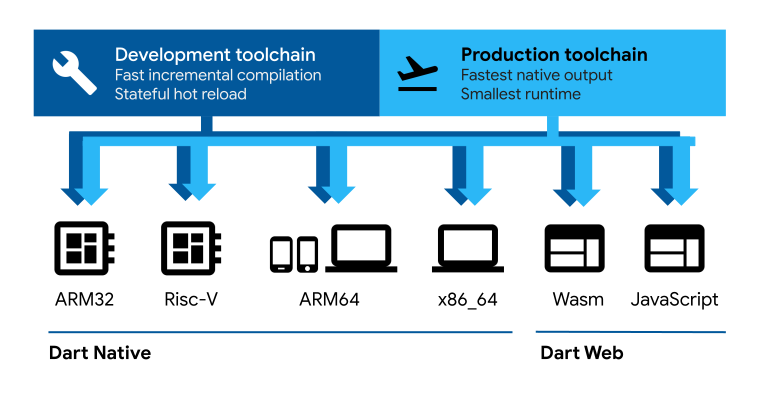
\includegraphics[width=1.0\linewidth]{./images/dart_platforms.png}
    \caption{Overview of all the devices that dart is able to reach.}
    \label{fig:dartPlatforms}
\end{figure*}

\noindent As we can see from \cref{fig:dartPlatforms}, the devices covered by a single code base range from embedded device architectures to mobile and laptop devices (by using Dart VM with just-in-time (JIT) compilation and an ahead-of-time (AOT) compiler) to web applications, with his web compiler that translate Dart into JavaScript or WebAssembly. Additionally, the language is type safe, so it uses static type checking to ensure that a variable's value always matches the variable's static type. This is done without sacrificing flexibility, since the language still permits the use of a dynamic type combined with runtime checks, which can be useful during experimentation or for code that needs to be especially dynamic, through the usage of the \texttt{dynamic} keyword. The language has also built-in null safety, so values can't be null unless the programmer explicitly say they can be. In this way dart can protect from null exceptions at runtime through static code analysis. Unlike other null-safe languages, this non-nullability is also retained at runtime, so if dart determines that a variable is non-nullable, that variable can never be null. The language also comes with a mature and complete \texttt{async-await} syntax for UI with event-driven code, all paired with a concurrency system based on dart isolates (separates memory-isolated threads of execution used to achieve concurrency). Dart comes with a rich set of libraries, ranging from core libraries (\texttt{dart:core}) from the ones to parse json (\texttt{dart:convert}), for concurrency (\texttt{dart:isolate}), web (\texttt{package:web}) and so on \cite{Dart}.

\subsubsection{Javascript}

\begin{wrapfigure}{l}{0.18\textwidth} % 'l' for left alignment, width of the wrapped area
    \captionsetup{font=footnotesize}
    \centering
    
\includegraphics[width=\linewidth]{images/javascript.png}
    \caption{Logo of the Javascript\\Language.}
\end{wrapfigure}

Javascript is a high-level, often just-in-time compiled language that represents the core technology to build web applications. Among his characteristics has dynamic typing, prototype-based object-orientation, and first-class functions. It is multi-paradigm, supporting event-driven, functional, and imperative programming styles. It comes with APIs to work with text, dates, regular expressions, standard data structures, and the Document Object Model (DOM). JavaScript is a single-threaded language, based on the event loop approach. The runtime processes messages from a queue one at a time, and it calls a function associated with each new message, creating a call stack frame with the function's arguments and local variables, which will shrink and grow based on the function's needs. When the call stack is empty and the function completed, javascript proceeds to the next message in the queue. In order to execute javascript code, a software component that executes the code called javascript engine is needed. These engines are tipically developed by web browser vendors: infact, they tipically provide a runtime system, to enable interaction with a broader environment. The runtime system includes the necessary APIs for input/output operations, such as networking, storage, and graphics, and provides the ability to import scripts \cite{Javascript}.

\subsubsection{Groovy}

\begin{wrapfigure}{l}{0.18\textwidth} % 'l' for left alignment, width of the wrapped area
    \captionsetup{font=footnotesize}
    \centering
    
\includegraphics[width=\linewidth]{images/groovy.png}
    \caption{Logo of the Groovy\\Programming\\Language.}
\end{wrapfigure}

Groovy is an object-oriented programming language, with dynamic typing for the Java Platform, alternative to the Java language. It can also be employed as a scripting language, intended to manage application automations for the Java Platform. The language also has features similar to languages such as Python, Ruby, Perl, and Smalltalk. Based on the Java platform, the language uses a Java-like syntax, based on curly brackets and is dynamically compiled in bytecode via the Java Virtual Machine. The Groovy compiler can be used to generate standard Java bytecode to interoperate seamlessly on any Java project. Among his features, the interoperability with java (java files are valid groovy files) makes him very versatile, but groovy code can be more compact. It is characterized by object-oriented features (like operator overloading and polymorphic iteration) as well as safe navigation operator \texttt{?.} to check automatically for null pointers. The latest versions add the support to newer features like modularity, static compilation, type checking and mullticatch blocks. Groovy has also native support of markup languages such as XML and HTML by using an inline Document Object Model (DOM) syntax. A Groovy script is fully parsed, compiled, and generated all before execution (similarly to Pyrthon and Ruby) and differently from Java, a groovy source code file can be executed as an uncompiled script under some circumstances\cite{Groovy}. Groovy is also used in the Gradle build system (see \cref{subsubsec:gradle}), which is the official build system for Android applications, and it is used to define the build configuration and dependencies for the android part of the project.  

% \subsubsection{Ruby}

% \begin{wrapfigure}{l}{0.18\textwidth} % 'l' for left alignment, width of the wrapped area
%     \captionsetup{font=footnotesize}
%     \centering
%     
\includegraphics[width=\linewidth]{images/ruby.png}
%     \caption{Logo of the Ruby\\Programming\\Language.}
% \end{wrapfigure}

% Ruby is an high-level, interpreted and general-purpose programming language, designed by having in mind the programmer productivity, simplicity and fun, but also minimizing programmer work and possible confusion. In Ruby, everything is an object, also primitive data types. The language is dynamically typed, uses garbage collection and just-in-time compilation and it is a multi-paradigm programming language by allowing procedural, object-oriented, and functional programming. Since in ruby everything is an object, everything has certain built-in abilities called methods. Every function is a method, methods are always called on an object and methods defined at the top level scope become methods of the object class. Ruby also supports inheritance with dynamic dispatch, mixins and singleton methods, but does not support multiple inheritance. However there is still the possibility for classes to import modules as mixins. Among its other most relevant features we have dynamic and duck typing which allows variables to hold objects of any type and change types at runtime, garbage collection that automatically manages memory, reducing the need for manual memory management and helping prevent memory leaks. Also robust exception handling mechanisms are provided using \texttt{begin,rescue,ensure} and \texttt{raise}, allowing developers to gracefully handle runtime errors, and operator overloading, giving the possiblity to redefine the behavior of operators for their custom classes, providing more intuitive and readable code. Finally, concurrent programming support is enabled through native thread and fibers and a package manager (called RubyGems) is used to provide a standardized way to distribute, install, and manage Ruby libraries and applications\cite{Ruby}. Ruby is also used in the CocoaPods build system (see \cref{subsubsec:cocoapods}), which is the official build system for iOS applications, and it is used to define the build configuration and dependencies for the iOS part of the project.

\newpage
\subsubsection{Yaml for flutter pub package manager}

\begin{wrapfigure}{l}{0.18\textwidth} % 'l' for left alignment, width of the wrapped area
    \captionsetup{font=footnotesize}
    \centering
    
\includegraphics[width=\linewidth]{images/yaml.png}
    \caption{Logo of the Yaml\\Language.}
\end{wrapfigure}

YAML is a data serialization language that is human readable. His common usage regards configuration files and applications where data is being stored or transmitted. The language targets many of the same communications applications as Extensible Markup Language (XML) but his minimal syntax differs from Standard Generalized Markup Language (SGML). The language also supports JSON style inside the same file. In Yaml custom data types are allowed but tipically they are not needed, since the language natively encodes scalars (strings, integers, and floats), lists, and associative arrays (so maps, dictionaries or hashes) all based on the Perl language. In particular, there is the possibility for both lists and associative arrays to form nested structures. It reuses escape sequences like in C and uses whitespace wrapping for multi-line strings like in HTML. Read and write support of Yaml is available for many programming languages and editors, where their extension is tipically \texttt{.yaml} or \texttt{.yml}. Regarding the syntax, whitespace indentation is used for denoting structure like in Python and typically uses UTF-32 encoding in order to have JSON compatibility. It is possible to comment a line with the \texttt{\#} character, use strings with single or double quotes, and specify lists and arrociative arrays respectively through square brackets (\texttt{[...]}) or curly braces (\texttt{\{...\}})\cite{Yaml}. In the project, Yaml is used to define the dependencies in the \texttt{pubspec.yaml} file, which is the configuration file for the Flutter pub package manager (see \cref{subsubsec:pub}).

\newpage
\subsection{Automation Dependencies Tools}
% While dependency management on the project was mainly done by using the pub package manager (see \cref{subsubsec:pub}), native Android/iOS plugins require Gradle (Android) and CocoaPods (iOS) behind the scenes as additional tools. In this section these tools and their functionalities will be covered.

\subsubsection{Pub Package Manager}
\label{subsubsec:pub}

For managing flutter dependencies in our project, the pub package manager has been employed. It uses a \texttt{.yaml} file (pubspec.yaml) to list the dependencies and has a command-line interface that works both for flutter framework and dart programming language (in our case we exploited it with flutter). The syntax is relatively simple and it works by using the \texttt{pub} command followed by a subcommand. \newline There are several subcommands that are divided into three main categories, based on functionalities\cite{Pub}:
\vspace{3ex}
\begin{itemize}[nosep]
    \item \textbf{Managing Package Dependencies:} in this category the most relevant are the \texttt{get} or \texttt{upgrade} commands, that respectively fetch or upgrade the dependencies that are used by a package. Also other commandss are available, like \texttt{downgrade} to downgrade the dependencies at their lowest version for testing, or dually \texttt{upgrade} that upgrades the dependencies to their highest version. 
    \item \textbf{Running command-line apps:} in this category fall the \texttt{global} command, which allows to make a package globally available, so that is possible to run scripts from his bin directory (the directory must also be added to the PATH variables).
    \item \textbf{Deploying packages and apps:} the \texttt{publish} command here is used to share developed dart packages with the community. This is done by uploading the package to the \href{https://pub.dev/}{pub.dev website}, acting as a package repository where all developer can download the published packages. 
\end{itemize}

\newpage
\subsubsection{Gradle}
\label{subsubsec:gradle}

\begin{wrapfigure}{l}{0.18\textwidth} % 'l' for left alignment, width of the wrapped area
    \captionsetup{font=footnotesize}
    \centering
    
\includegraphics[width=\linewidth]{images/gradle.png}
    \caption{Logo of the Gradle\\Automation\\Tool.}
\end{wrapfigure}

For managing dependencies/plugins in our project on the android side, gradle has been employed. Gradle is a build automation tool for software development which uses either Groovy or Java/Kotlin as language (in our case we leveraged on Groovy). It offers support for all phases of a build process, from compilation to verification, dependency resolving but also test execution, source code generation, packaging and publishing. Gradle is a multi-language tool, supporting languages like Java, Kotlin, Groovy, Scala, C, C++ and Javascript. Gradle operates with his own domain-specific language in contrast with the maven approach with XML. It has been designed to handle multi-project builds, that can be very large. Infact, it supports a series of build tasks that can run serially or in parallel, and build components can be also cached. Regarding his main features, gradle follows a convention (folder structure of the project, standard tasks and their order as well as dependency repositories) over configuration approach, all the build phases can be described in short configuration files. All conventions can still be overriden if it is necessary. One crucial gradle component is the plugin, that allow to integrate a set of configurations and tasks into a project, and can be either downloaded from a central plugin repository or custom-developed\cite{Gradle}.

\begin{figure*}
    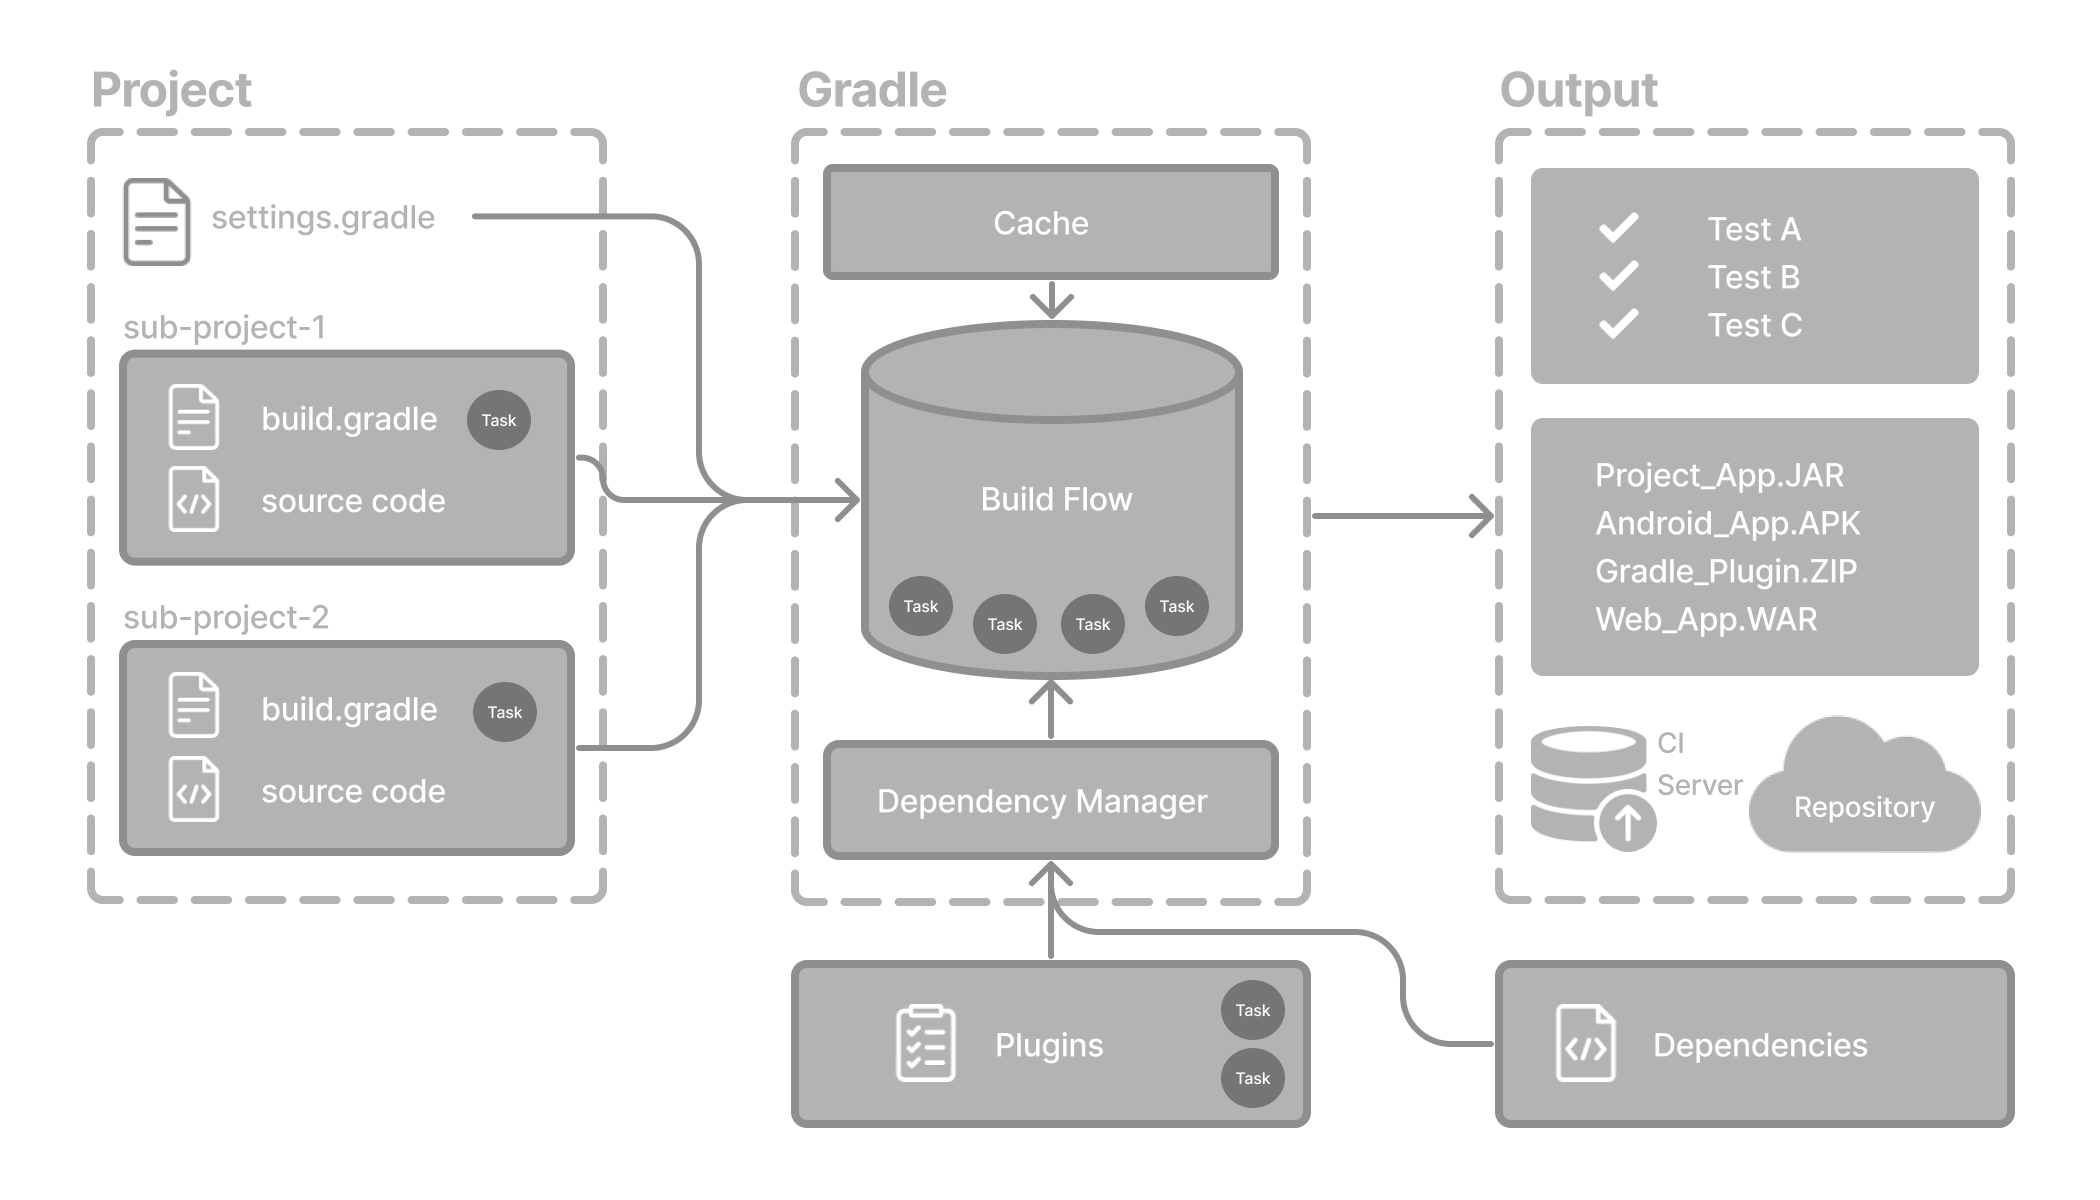
\includegraphics[width=1.0\linewidth]{./images/gradle_basics.png}
    \caption[Gradle operating flow.]{Gradle operating flow \protect\cite{GradleBasics}.}
    \label{fig:gradleBasics}
\end{figure*}

\subsubsection{Npm}

\begin{wrapfigure}{l}{0.18\textwidth} % 'l' for left alignment, width of the wrapped area
    \captionsetup{font=footnotesize}
    \centering
    
\includegraphics[width=\linewidth]{images/npm.png}
    \caption{Logo of the NPM\\Automation\\Tool.}
\end{wrapfigure}

For managing dependencies/plugins in our project on the web side, npm has been employed. Npm is a package manager for the JavaScript programming language and the default package manager for the JavaScript runtime environment Node.js. It consists of a command line client interface and an online database of public and paid-for private packages, called the npm registry. The command line client interface allows users to consume and distribute JavaScript modules that are available in the registry and the available packages can be browsed and searched via the npm website. When used as a dependency manager for a local project, npm can install, in one command, all the dependencies of a project through the \texttt{package.json} file. Inside this file each dependency can specify a range of valid versions: this to allow developers to auto-update their packages and at the same time avoiding unwanted breaking changes. Npm also provides the \texttt{package-lock.json} file which has the entry of the exact version used by the project after evaluating semantic versioning in package.json.  \cite{NPM}.

% \newpage
% \subsubsection{CocoaPods}
% \label{subsubsec:cocoapods}

% \begin{wrapfigure}{l}{0.18\textwidth} % 'l' for left alignment, width of the wrapped area
%     \captionsetup{font=footnotesize}
%     \centering
%     
\includegraphics[width=\linewidth]{images/cocoapods.png}
%     \caption{Logo of the CocoaPods\\Dependency\\Manager.}
% \end{wrapfigure}

% For managing dependencies/plugins in our project on the android part of the project, cocoapods has been employed. CocoaPods is an application level dependency manager for Objective-C, Swift and other languages that uses Objective-C as runtime (like RubyMotion), is written in Ruby and uses it to manage the dependencies. It provides a standard format for managing external libraries and is inspired by the RubyGems and Bundler combination. CocoaPods is executed through the command line and installs the application dependencies by specifying them rather than copying source files. The dependencies are specified into a text file (Podfile). CocoaPods will then recursively resolves dependencies between libraries and then fetch the needed source code. His dependency resolution system is powered by Molinillo, which is also used by other large projects such as Bundler and RubyGems\cite{CocoaPods}.

% \begin{figure}[h]
%     \centering
%     \begin{lstlisting}[
%         language=, % Leave empty since it is not a predefined language
%         basicstyle=\ttfamily,
%         keywordstyle=\color{blue},
%         commentstyle=\color{green},
%         stringstyle=\color{red},
%         showstringspaces=false,
%         breaklines=true,
%         frame=none, % No border
%         numbers=none % No line numbers
%     ]
%     platform :ios, '13.0'
%     use_frameworks!

%     target 'MyApp' do
%         pod 'Alamofire', '~> 5.6'
%         pod 'SwiftyJSON', '~> 5.0'

%         target 'MyAppTests' do
%             inherit! :search_paths
%         end
%     end
%     \end{lstlisting}
% \end{figure}

% \noindent As a practical example this POD file can be considered. It sets the minimum iOS version, enables frameworks, and adds Alamofire and SwiftyJSON as dependencies to handle networking and JSON parsing respectively.

\subsection{Integrated Development Environment}

\begin{wrapfigure}{l}{0.18\textwidth} % 'l' for left alignment, width of the wrapped area
    \captionsetup{font=footnotesize}
    \centering
    
\includegraphics[width=\linewidth]{images/android_studio.png}
    \caption{Logo of the Android\\Studio IDE.}
\end{wrapfigure}

As Integrated Development Environment for the mobile application, Android Studio has been employed. Android Studio is the official IDE for Android app development, but it seamlessly supports flutter through the flutter plugin. Based upon JetBrains' IntelliJ IDEA software, it inherite most of his features (like code completion, refactoring, debugging but also built-in tools and a plugin ecosystem). These features, combined with the fact that it is available for download for windows, macOs and linux, has helped to make it one of the most used IDE (together with VsCode) on this field. Android Studio is licensed under the Apache license but it ships with some SDK updates that are under a non-free license, so it is not completely open source. The supported languages are Java, Kotlin (the actual Google's preferred language for Android app development), C++ and more with extensions, such as Go and Dart\cite{AndroidStudio}. 

\newpage
\subsubsection{Core features}
% compose design tools alla fine dato che esula un po
Several are the core features, based on IntelliJ Idea and then further extended and enriched, that made this IDE a de-facto standard on mobile development:

\noindent The \textbf{Intelligent code editor features} have been further extended to enhance the developers productivity. Particularly focused on the Android side, there is a clean \textit{Project Structure}, where each project contains one or more modules (Android App, Library and Google App Engine Modules), each one with source code files and resource files. The Android App module in particular then contains the manifest, the source code and then all the non-code resources in the \texttt{res} folder. Then, regardless of the mobile platform, Android Studio includes \textit{Debug and profile tools} that help in debugging and improving the performance of code, including inline debugging and performance analysis tools. It is possible to leverage on inline debugging to enhance code walkthroughs in the debugger view with inline verification of references, expressions, and variable values. Also the Performance Profiler allows to easily track memory and CPU usage, find deallocated objects, optimize graphics performance, locate memory leaks and analyze network requests. The Memory Profiler can be used instead to track memory allocation and watch where objects are being allocated when you perform certain actions, since can be useful to optimize the app performance and memory use by adjusting the method calls. Also heap dump is allowed in a specific format, to analyze memory usage and find memory leaks. A solid Code Inspection system is also provided. At compile time, the IDE automatically runs configured lint checks and other IDE inspections to help you easily identify and correct problems with the code quality. The lint tool checks the project source files for potential bugs and optimization improvements for correctness, security, performance, usability, accessibility, and internationalization. In addition to that, IntelliJ code inspections validates annotations to streamline coding workflow. Finally, there is a Log System to view adb output and device log messages when building or running the app and also an Annotation System is supported to annotate variables, parameters, and return values to help find bugs, such as null pointer exceptions and resource type conflicts \cite{AndroidStudioCodeEditorFeature}.

\noindent The \textbf{Flexible Gradle Build System} is employed, with specific Android capabilities provided by the Android Gradle Plugin. Leveraging on the Gradle flexibility allows us to easily manage dependencies, than also customize, configure, and extend the build process, as well as create multiple APKs. All this without modifying the app core source files, only the gradle files (either using groovy or kotlin). By going deeper into the build system it is possible to clearly distinguish some of the main aspects: the \textit{build types}, that define certain properties that Gradle uses when building and packaging your app (for example, the debug build type enables debug options and signs the app with the debug key, while the release build type signs your app with a release key for distribution). At least one build types must be defined and the IDE creates debug and release build types by default; The \textit{product flavors} that are different versions of your app (like free and paid one) that can be released to users: they can be customized to use different code and resources while sharing the common parts. The \textit{dependencies} are managed through the local file system and remote repositories: this eliminates the nedd to manually search, download, and copy binary packages into the project. Related to the APKs, the \textit{Code and resource shrinking tool} allow to  shrink code and resources by using its built-in shrinking tools and applying the appropriate set of rules: as result the APK size may be reduced significantly. Finally, the \textit{multiple APK support} allows to automatically build different APKs that contains only the code and resources needed for a specific screen density or Application Binary Interface (ABI)\cite{AndroidStudioBuildSystemFeature}.

\noindent \newline The \textbf{Android Emulator} simulates Android devices on the computer so that it is easy to test an application on a variety of devices and Android API levels without needing to have each physical device. In most cases, the emulator is the best option to test an application on Android (alternatively it is possible to deploy the application on a physical device). Use the Emulator offers \textit{flexibility}, since it is able to simulate lots of devices and comes also with predefined configurations for Android phone, tablet, Wear OS, Android Automotive OS, and Android TV devices. It also offers \textit{high fidelity} because it offers almost all capabilities of a real android device, sich as phone calls, messages, location, play store, networks, sensors and much more. Finally, on some aspects (like data trasfer) it is possible to gain \textit{speed}, since data tranfer is higher to the emulator compared with a real device speed on USB. Each instance of the Android Emulator uses an Android virtual device (AVD) to specify the Android version and hardware characteristics of the simulated device and each AVD work as a separate device (it is treated independently from the others). Each AVD's data is stored inside a specific directory (directory then used to load the data when booting it up). It is also possible to test an application with WearOs Devices by using the Wear OS pairing assistant that provides a step-by-step guide through pairing Wear OS emulators with physical or virtual phones directly in the IDE. Use the emulator is pretty simple: it is possible to simulate the touch with the mouse in the same way and use the provided buttons on the emulator panel for additional functionalities\cite{AndroidStudioEmulatorFeature}.

\begin{figure*}
    \centering
    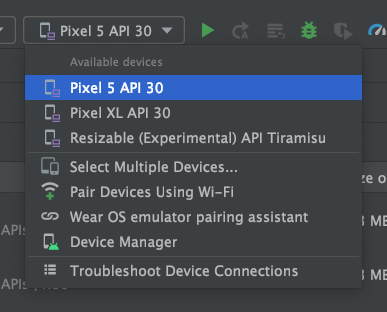
\includegraphics[width=0.6\linewidth]{./images/target_devices_dropdown.png}
    \caption[The target device menu.]{The target device menu\protect\cite{AndroidStudioEmulatorFeature}.}
\end{figure*}

\noindent The \textbf{APK Analyzer} gives more insight into the APK/Android Bundle composition once the build has been completed. By leveragin on this tool it is possible to reduce the debugging time related to DEX files and resources in the app and help reduce the APK size easily. APKs are files that follow the ZIP file format, and the APK Analyzer \textit{displays each file or folder} as an expandable entity that can be used to to navigate into folders. For each entity three metrics are shown: Raw File Size (entity contribution to the total APK size), Download Size (estimated compressed size of the entity as it would be delivered by Google Play) and the percentage of Total Download Size (how much that entity impact on the overall APK size). The tool also allow to \textit{view the AndroidManifest.xml} file, to understand any changes that might have been made to your app during the build. For example, since product flavors and libraries have their own manifest file, this is then merged with the appllication one and the tool helps in visualizing it. It also provides some lint capabilities, with warnings or errors that appear in the top-right corner. The APK Analyzer also provides a \textit{DEX file viewer} that allows to see underlying information in the DEX files (class, package, total reference, and declaration counts), which can assist in deciding whether to use multidex or how to remove dependencies to get below the 64K DEX limit (Also the possibility to Filter the DEX file tree view is provided). Through the APK Analyzer there is also the possibility to \textit{see code, resource entities and textual/binary files} inside the final APK, since during the build process shrinking rules can alter the code, and image resources can be overridden by resources in a product flavor. Finally, the tool allows to \textit{compare different files}: specifically, the tool allows to compare the size of the entities in two different APK or app bundle files, and this is particularly useful to understand why the app increased in size compared to a previous release\cite{AndroidStudioAPKAnalyzerFeature}.

\begin{figure*}
    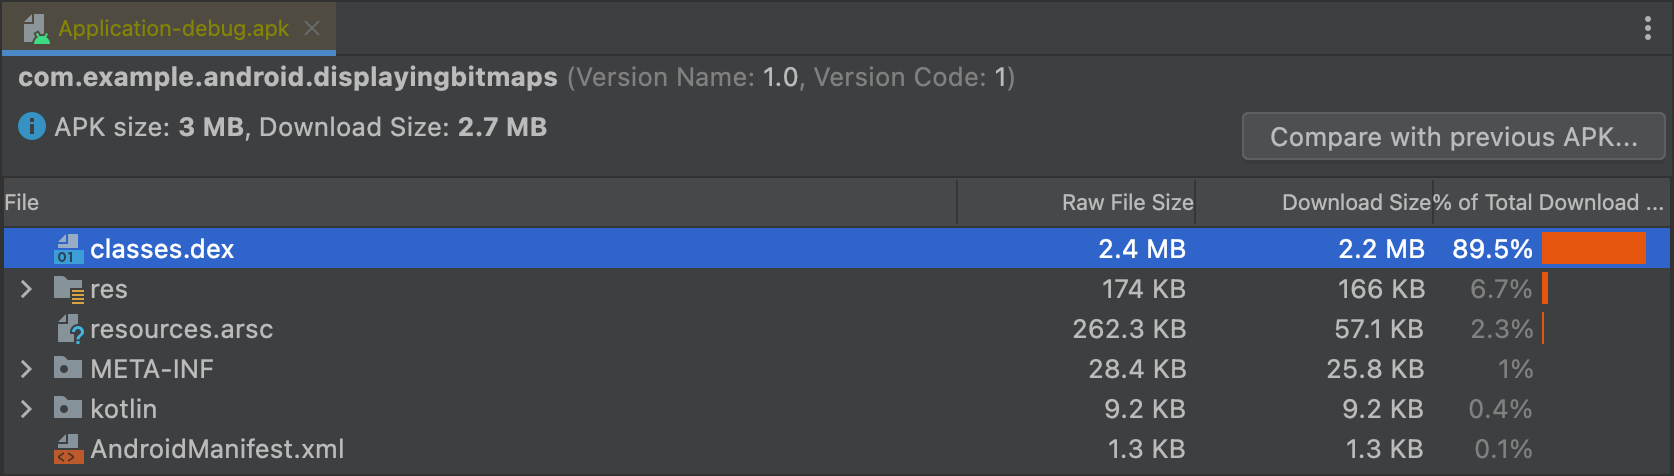
\includegraphics[width=1.0\linewidth]{./images/apk_file_sizes.png}
    \caption[File sizes in the APK Analyzer.]{File sizes in the APK Analyzer\protect\cite{AndroidStudioAPKAnalyzerFeature}.}
\end{figure*}

\subsubsection{New features}

As a result of the massive involvement of artificial intelligence and cloud computing, by moving all into the cloud, also Android Studio has adapted by integrating two new major features into the IDE\cite{AndroidStudioNewFeatures}:

\begin{itemize}[nosep] % 'nosep' removes extra spacing between items
    \item \textbf{Gemini}, coding assistant powered by artificial intelligence, that can understand natural language. Helps into achieving more productivity by generating code, finding relevant resources, learning best practices. However it has to be said that like any AI model, sometimes might provide inaccurate, misleading, or false information while presenting it confidently.
    \item \textbf{A Web Version} of the IDE (in early access preview), that leverages on IDX (web-based workspace for full-stack application development made by google itself). It could be used as a convenient way to open up samples but also open an existing project on Github inside the browser.
\end{itemize}

\begin{figure*}
    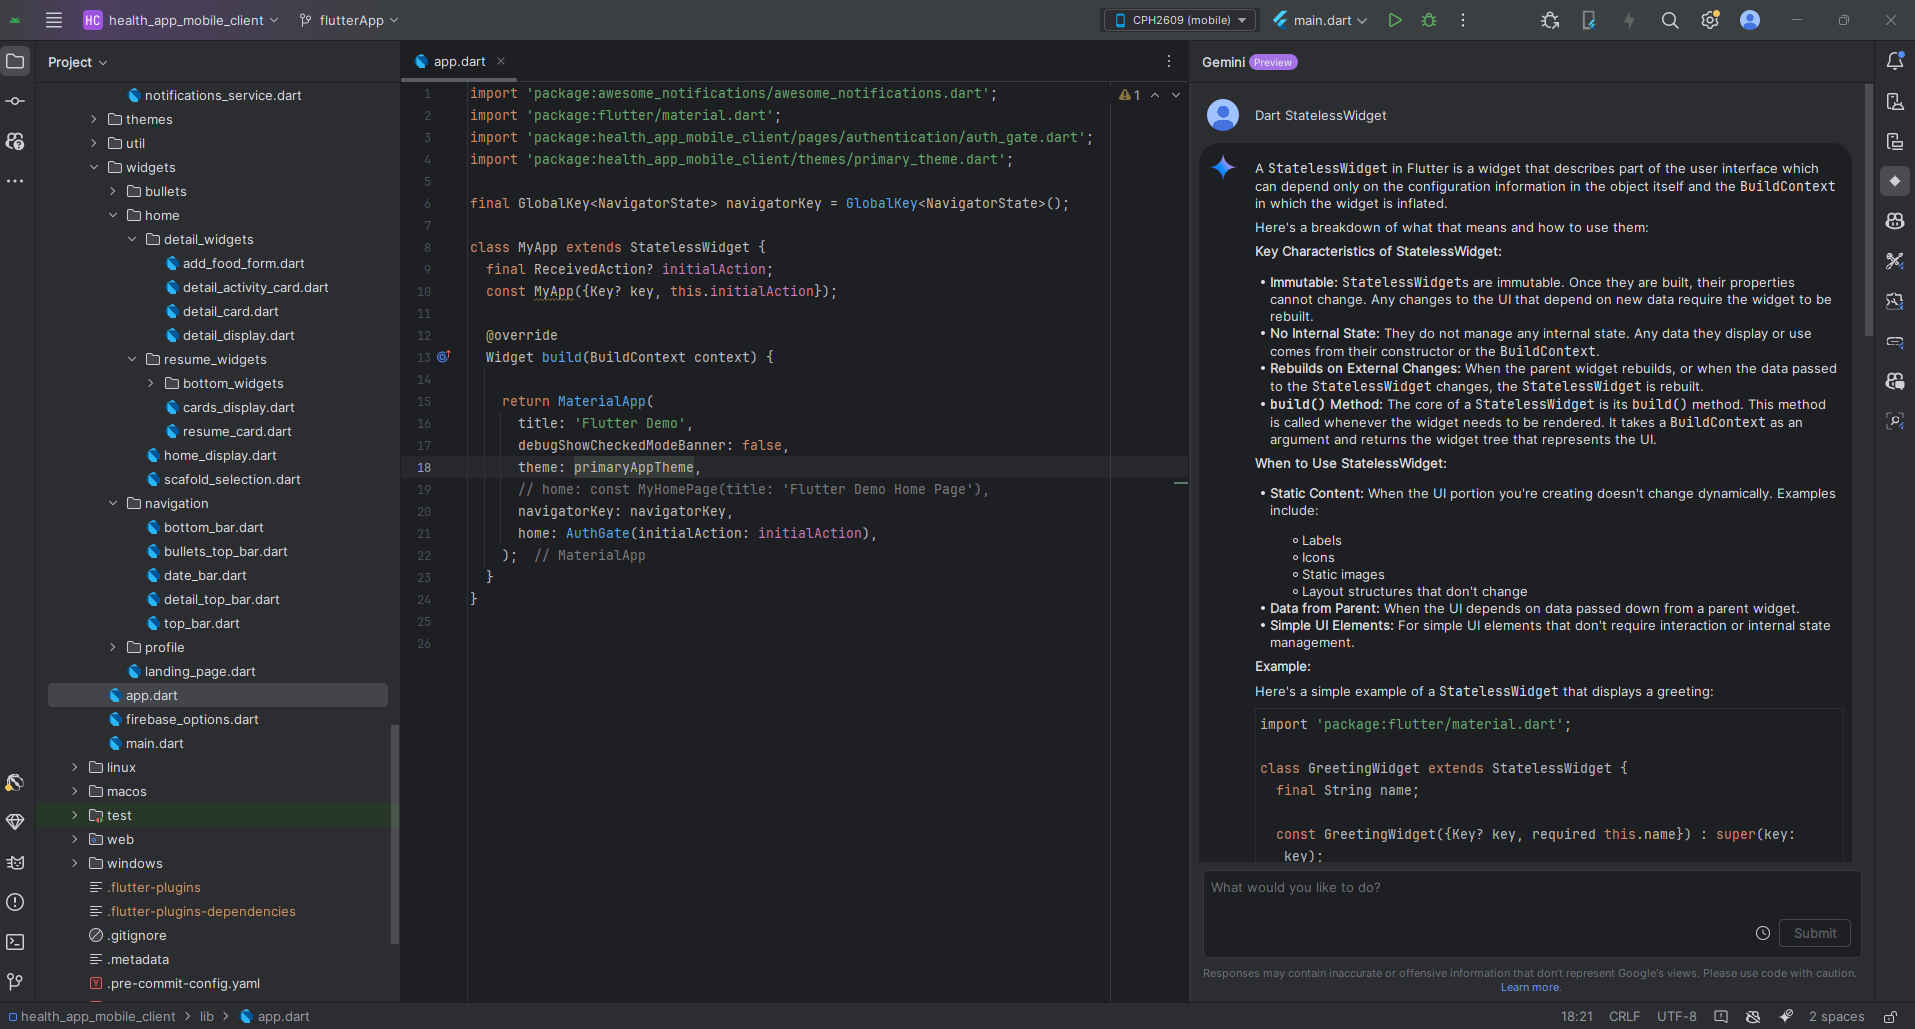
\includegraphics[width=1.0\linewidth]{./images/gemini.png}
    \caption{Example of the Gemini feature usage through the tab in android studio.}
\end{figure*}

\subsection{Code Editor}

\begin{wrapfigure}{l}{0.18\textwidth} % 'l' for left alignment, width of the wrapped area
    \captionsetup{font=footnotesize}
    \centering
    
\includegraphics[width=\linewidth]{images/vs_code.png}
    \caption{Logo of the VsCode\\Code Editor.}
\end{wrapfigure}

In order to develop the web application part of the system, VsCode was employed. VsCode is a fully-customizable code editor that streamline the development experience with features like IntelliSense, debugging and web version. It allows to install extensions to add additional services and customize itself. VsCode is fully customizable, with the possibility to change theme colors and defining customization profiles and easily switch between them. Also sync settings across VsCode instances on different devices is possible. It supports almost every major programming language and given to his lightweight nature and portability, can run also on the web browser. It comes also with a built-in terminal and git version control support, and more recently also artificial intelligence support was added through the copilot extension, that allows to edit multiple file through copilot, given a description of what we want to build as well as giving code suggestions, that can be either accepted or rejected \cite{VsCode}. 
\newpage
\subsection{Google Firebase}
Google Firebase is a backend comprehensive solution that allows to build, deploy and run an application. It comes with already-made extensions for common use cases, and it is easy to integrate on iOS, Android, and Web. It is a platform developed by Google, composed of several services, each one with a specific purpose: the employed services used for satisfy the system requirements will be covered.
\subsubsection{Authentication Service}
The Firebase Authentication service allows to perform a simple, multi-platform sign-in by providing backend services, easy-to-use SDKs, and ready-made UI libraries to authenticate users. It provides an easy authentication system by supporting several platforms and authentication methods (email and password accounts, phone auth, and Google, Apple, Facebook and more). It also simplifies the sign-in and onboarding experience for end users thanks to FirebaseUI Auth component, that implement the best practices for authentication on mobile devices and websites. It allows to setup a working authentication system for an application in under 10 lines of code, including account merging, and applies Google's internal expertise into adopting a comprehensive security system \cite{FirebaseAuthentication}.
\subsubsection{Cloud Firestore Database}
The Cloud Firestore Database service is a NoSQL document database that allows to store, sync, and query data for an application on a global scale. Given the fact that is a NoSQL database, it lets strcture the data freely with collections and documents and easily retrieve them by using expressive queries. It allows to build serverless app through a mobile and web SDKs and a comprehensive set of security rules, but it still provide support for traditional client libraries like Node and Python. It comes with a notification system that communicates data changes to easily build collaborative experiences and realtime apps, and also with an offline mode so that users can change their data at any time. The system (powered by Google's storage infrastructure) is fully scalable, allowing to focus on the application without worrying about servers and consistency. Finally, the declarative security language and the integration with firebase authentication allows to setup a strong user-based security \cite{CloudFirestore}.
\subsubsection{Cloud Storage}
The Cloud Storage is a powerful, simple, and cost-effective service that allow through the client SDKs to store images, audio, video, or other user-generated content. Is designed to store and serve contents quickly and easily. It is a scalable service, allowing to effortlessly grow from prototype to production and automatically scale up computing resources with cloud functions. Also with this service, a strong user-based security is enforced with an integration with firebase authentication through the SDK APIs for Cloud Storage \cite{CloudStorage}.
\subsubsection{Performance Monitoring}
The Performance Monitoring service, available both for mobile and web applications, allows to measure app network requests, screen rendering times, as well as custom and automated traces and gain insights of the app performance. This tool allows to keep track of the permormance on different app versions as new features are delivered or configuration changes are made, with a dashboard that makes easy to focus on the most important metrics. A monitoring of data like app version and device allows to understand how the app performs from the users' point of view. There is the possibility to closely monitor HTTP/S requests by analyzing response time, success rate as well as payload size, particularly useful for critical requests. Thanks to that, understand where performance issues take place and address them is easier \cite{PerformanceMonitoring}.
\subsubsection{Crashlytics}
The Crashlytics service, integrable with mobile and unity apps, allows to obtain a real time crash and error report and analysis to help keep the apps running flawlessly. The tool starts capturing crashes and groups them into manageable issues based on the impact on real users,so that it is easier to prioritize what to fix first. AI-powered insights helps understand why a crash happened and help to get to the root cause faster. Crashlytics works seamlessly with industry-standard tools including Jira, Slack, BigQuery, and with integrations for Android Studio it is possible to view the data directly in the IDE, making it easy to debug crashes. Contextual informations about the crashes are displayed, like the timeline of events leading up to app crashes to quickly reproduce bugs and uncover the root cause \cite{Crashlytics}.

\subsection{Dependencies}
This section will cover the major dependencies with a focus on background features and firebase that have been used in the project.

% \subsubsection{fl\_chart}
% The first library employed was fl\_chart, used to implement data visualization through the usage of intuitive charts. The library is highly customizable and supports several types of chart, like bar chart, pie chart, scatter chart ,line and multiline chart and radar chart. Among them we mainly employed bar, line and multiline chart for our purposes. The employed version is the 0.67.0.

% \begin{figure*}
%     \centering
%     \begin{minipage}{0.3\linewidth}
%         \centering
%         \includegraphics[width=\linewidth]{./images/bar_chart_sample.png}
%     \end{minipage}
%     \begin{minipage}{0.3\linewidth}
%         \centering
%         \includegraphics[width=\linewidth]{./images/line_chart_sample.png}
%     \end{minipage}
%     \begin{minipage}{0.3\linewidth}
%         \centering
%         \includegraphics[width=\linewidth]{./images/multiline_chart_sample.png}
%     \end{minipage}
%     \caption[Example of the three main chart types employed in the application.]{Example of the three main chart types employed in the application. \protect\cite{FlChart}.}
%     \label{fig:three_images}
% \end{figure*}

\subsubsection{health}
The health library was used to fetch health data from the devices to successfully use them. This library is a wrapper for Apple's HealthKit on iOS and Google's Health Connect on Android, and enables reading and writing operations from/to Apple Health and Google Health Connect. All the library functionalities are managed through a singleton \texttt{Health} instance, which supports lots of operations. \newline However, for our purposes, we mainly exploited: 

\begin{itemize}[nosep] % 'nosep' removes extra spacing between items
    \item Permission handling operations to access health data, through the \texttt{hasPermissions} method to check the permissions and the \texttt{requestAuthorization} method to request them.
    \item Read operations (through the \texttt{getHealthDataFromTypes} method) to read the needed health data.
\end{itemize}

\noindent No write operations have been adopted, as the wearables or applications adopted by the users are synchronized and write data directly to Google's Health Connect, since it constitute the standard: from it health will then retrieve the data. The employed version is the 11.1.0 \cite{Health}.

\subsubsection{workmanager}
The workmanager library, used to perform the health data backup (see \cref{tab:fr3} FR 3.4), is a powerful solution for managing background tasks in Flutter applications. It allows to schedule and execute tasks even when the app is not actively running, useful for tasks such as periodic data synchronization, notifications, and other background operations. The package provides a simple API to schedule background tasks at specific intervals or under certain conditions, with the possibility to specify retry policies for failed tasks, ensuring robustness in the face of temporary issues. These tasks are executed efficiently, having minimal impact on the device resources and battery life. The employed version is the 0.5.2 \cite{Workmanager}.
\subsubsection{awesome\_notifications}
The awesome notifications library, used to implement the notification system for the users (see \cref{tab:fr2} FR 3.4), allows to implement custom local and push notifications on Flutter with real-time events. It allows to keep the user ingaged, thanks to the possibility of creating notifications with different layouts, images, sounds and so on. Real-time events are deelivered at Flutter level code, leaving the possibility to the programmer to handle them. It gives the possibility of scheduling periodic or single notifications, is easy-to-use and highly customizable, including also the possibility to translation (see \cref{tab:nfr} NFR8). The employed version is the 0.10.0 \cite{AwesomeNotifications}.
\subsubsection{firebase}
Regarding firebase, given the variety of services that it offers, several dependencies have been employed in the project to cover all the functionalities needed:

\begin{itemize}[nosep] % 'nosep' removes extra spacing between items
    \item \textbf{firebase\_core\:} the base dependency for the firebase services, and it is required to use the Firebase Core API, which enables connecting to multiple Firebase apps. The employed version is the 3.6.0.
    \item \textbf{firebase\_auth\:} dependency enabling classic authentication with email/password as well as identity providers like Google, Facebook and Twitter through the Firebase Authentication API. The employed version is the 5.3.1.
    \item \textbf{firebase\_ui\_auth}, a dependency that provides pre-built widgets, already integrated with the variety of the Firebase Auth providers. The employed version is the 1.10.0.
    \item \textbf{firebase\_ui\_oauth\_google}, a dependency that allows to authenticate with Google through Oauth protocol, by spcifying it as authentication provider. The employed version is the 1.12.14.
    \item \textbf{firebase\_storage\:} dependency for Firebase Cloud Storage service, allowing to easily store and retrieve files from it through the Firebase Cloud Storage API. The employed version is the 12.3.4.
    \item \textbf{firebase\_crashlytics\:} dependency for Firebase Crashlytics that allows, through the Firebase Crashlytics API usage, to report uncaught errors to the Firebase console. The employed version is the 4.3.3.
    \item \textbf{firebase\_performance\:} dependency for Google Performance Monitoring for Firebase, allowing to monitor traces and HTTP/S network requests and their parameters (like response time) through the Firebase Performance API. The employed version is the 0.10.1+3.
\end{itemize}

\noindent Regarding the related web application dependencies, only the \textbf{firebase} dependency has been employed, giving access to both authentication and cloud firestore database, in order to perform the operations. The employed version is the 11.3.1.

% \subsubsection{Health Connect}
